% -*- TeX:UK -*-
\chapter{Circular data}
\begin{refsection}
\label{text:circular}

\abstract{There are data whose scale is not on a number ray, but on a circle. Examples include angles on the windrose, hour of day and season of year. Special statistical tools are required to describe such data because of cross-over problems.   }

Consider, for example, measurements of flight direction of birds enroute to their summer quarters. These will scatter around \ang{0} (northwards, at least on the northern hemisphere). For example, we have two measurements, \ang{5} and \ang{355}. If we try to calculate the arithmetic mean, we get \( \frac{\ang{5} + \ang{355}}{2} = \ang{180} \), that is due south! Obviously, this mean is not a good measure of position of the data set. What is the problem?  We conventionally assign \ang{0} to north, and go clockwise from there. \ang{360} is the same as \ang{0} again. Similarly, we start the day at 00:00:00 (midnight), and after 23:59:59 we end at 00:00:00 again. A maternity ward may be interested in the time of day when most deliveries occur, so they can provide the required resources (full circle = \SI{24}{h} = \SI{1440}{min}). On the other hand, a conservation biologist may have the same question about the time of year when birthing activities occur (full circle = \SI{1}{a} = \SI{365}{d}), so that appropriate protective measures can be instigated (\Foreign{i.e.}, road closures).

Thus, the data that are not on a number ray, but on a circle, require special methods for statistical description to avoid cross-over problems \parencite{Bat-81, Fis-93, Ber-09}. Such data may be described by the \textbf{\Name{von Mieses} distribution} \parencite{Mie-18}, the circular equivalent of the normal distribution. It is characterised by two parameters, the position \skalar{\mu} and the dispersion \skalar{\kappa}. The density function is
\begin{equation}
  f(\AbsVec{x} | \mu,\kappa) = \frac{1}{2\pi\ I_0(\kappa)}\ \mathrm{e}^{\kappa \cos(\theta-\bar{\theta})}, \bar{\theta} \in [0\ldots 2\pi], \kappa > 0
\end{equation}
where \( I_0(\kappa) = \frac{1}{2\pi} \int_{0}^{2\pi} \exp(\kappa \cos(\theta - \bar{\theta})) d\theta \) the modified \Name{Bessel}-function of 0th order. Here, as in the rest of this chapter, angles are in the unit \si{rad}, \( [0\ldots 2\pi] \).

\section{The interface}

The interface is:
\begin{lstlisting}[caption=Interface of unit Circular]
  UNIT Circular;

  INTERFACE

  USES math,                  // Free Pascal math UNIT
       crt,                   // Free pascal UNIT
       MathFunc,              // basic math functions
       Dynam,                 // dynamic data structures
       Complex,               // Complex numbers
       Vector,                // vector arithmetic
       Matrix,                // matrix algebra
       Correlations,          // correlation coefficients
       Deskript,              // descriptive statistics
       Stat,                  // statistical distributions
       Zufall;                // pseudo-Random numbers

  CONST CircleError : BOOLEAN = FALSE;
        Nintey = Const_pi / 2;          // 90° in rad

  { **************** description of a single data vector ***************** }

  PROCEDURE Transform (VAR Data : VectorTyp; FullCircle : float);

  FUNCTION MedianDirection (TransformedData : VectorTyp) : float;

  FUNCTION MeanVector (TransformedData : VectorTyp; p : word) : ComplexTyp;

  FUNCTION CircularVariance (R : float) : float;

  FUNCTION CircularStandardDeviation (R : float) : float;

  FUNCTION CircularDispersion (TransformedData : VectorTyp; Mean : ComplexTyp) : float;

  FUNCTION Kappa (R : float; n : WORD) : float;

  FUNCTION TrigonometricMoment (Data : VectorTyp; MeanAngle : float; p : WORD) : ComplexTyp;

  function CenteredMean(Moment : ComplexTyp) : ComplexTyp;

  FUNCTION CircularSkew (TransformedData : VectorTyp; Mean : ComplexTyp) : float;

  FUNCTION CenteredCircularSkew (Mean1, Mean2 : ComplexTyp) : float;

  FUNCTION CircularKurtosis (TransformedData : VectorTyp; Mean : ComplexTyp) : float;

  FUNCTION CenteredCircularKurtosis (Mean1, Mean2 : ComplexTyp) : float;

  FUNCTION ConfidenceInterval (R, delta : float; n : WORD) : float;

  { ****************************** random numbers ************************ }

  FUNCTION RandomVonMieses(mu, kappa : float) : float;

  FUNCTION RandomUniformCircular : float;

  { ********************* Tests for preferred direction ****************** }

  FUNCTION Rayleigh (MeanVectorLength : float; n : WORD) : float;

  FUNCTION HodgesAjne (TransformedData : VectorTyp; MeanAngle : float) : float;

  PROCEDURE ChiSqrTest (Data : VectorTyp; Direction : float;
            Sectors : WORD; VAR ChiSqr : float; VAR dgf : WORD);

  FUNCTION HomewardComponent (n : WORD; Mean : ComplexTyp;
           Expected : float) : float;

  FUNCTION Rao (TransformedData : VectorTyp) : float;

  PROCEDURE Kuipers (Data : MatrixTyp;   VAR K, U : float);

  PROCEDURE CalculateCumulativeFrequencies (Data : VectorTyp;
            FullCircle : float; VAR Result : MatrixTyp);

  FUNCTION OneSample (MeanAngle, R, delta, TestAngle : float; n : WORD) : BOOLEAN;

 { ****************************** grouped data *************************** }

  FUNCTION MeanVectorGrouped (Transformed : MatrixTyp;
           Difference : float) : ComplexTyp;


  { ******************** Compare two circular distributions ************** }

  PROCEDURE Difference (Data1, Data2 : VectorTyp;
                        VAR KuipersV, WatsonsUSqr : float);

  FUNCTION FTest (Data1, Data2 : VectorTyp) : float;

  FUNCTION Wilcoxon (Data1, Data2 : VectorTyp;
                     Direction1, Direction2 : float) : float;

  PROCEDURE WatsonWilliams (TransformedData1, TransformedData2 : VectorTyp);

  FUNCTION KruskalWallis (TransformedData1, TransformedData2 : VectorTyp) : float;

  { *********************** linear-bivariate Data ************************ }

  PROCEDURE DescribeBivariat (Data : MatrixTyp);

  { ******** linear dependent, circular independent Correlation ********** }

  FUNCTION CAssociation (CONST theta, Y : VectorTyp; VAR Sig : SignificanceType) : float;

  PROCEDURE CircularLinearCorrelation (const TransformedData, yData: VectorTyp;
                                       VAR Correlation : float; VAR Sig : SignificanceType);

  PROCEDURE LinearPeriodicRankCorrelation (const TransformedData, yData: VectorTyp;
                                           VAR Correlation, U : float);

  PROCEDURE TrigonometricPolynomial (const TransformedData, yData: VectorTyp;
                                     Periode : float);

  { ****** Correlation circular dependent and independent variable ******* }

  PROCEDURE PeriodicRankCorrelation (CONST alpha, beta : VectorTyp;
                                       VAR rPlus, rMinus : float);

  PROCEDURE CircularCircularCorrelation (Alpha, Beta : VectorTyp;
            VAR Correlation : float; var Sig : SignificanceType);

  { ********************************************************************** }

  IMPLEMENTATION

  VAR xMax       : WORD;
      ch         : CHAR;
\end{lstlisting}

\section{Transformation of circular data}

The following routine ensures that the value is in the range of a full circle, \( [0\ldots 2\pi] \).

\begin{lstlisting}[caption=limit datum to  0..2\textpi ]
  FUNCTION ModuloTwoPi (Datum : float) : float;

  VAR x : float;

  BEGIN
    x := Datum;
    WHILE (x > Const_2pi) DO x := x - Const_2pi;
    WHILE (x < 0.0) DO x := x + Const_2pi;
    Result := x;
  END;
\end{lstlisting}

The following routine transforms the data in a data vector to the range of a full circle, \( [0\ldots 2\pi] \). The variable \texttt{FullCircle} contains the length to which the data are standardised (say, \SI{24}{h} for a day).

\begin{lstlisting}[caption=Transformation to 0..2\textpi]
  PROCEDURE Transform (VAR Data : VectorTyp; FullCircle : float);

  VAR n, i  : WORD;
      Datum : float;

  BEGIN
    n := VectorLength(Data);
    FOR i := 1 TO n DO
       BEGIN
         Datum := GetVectorElement(Data, i) * Const_2pi / FullCircle;
         SetVectorElement(Data, i, ModuloTwoPi(Datum));
       END;
  END;
\end{lstlisting}

\section{Description of a single vector of circular data}

\subsection{Position}

\begin{figure}
 \caption{Circular mean by vector addition. For details see text. }
 \label{fig:CircMean}
 \centering
 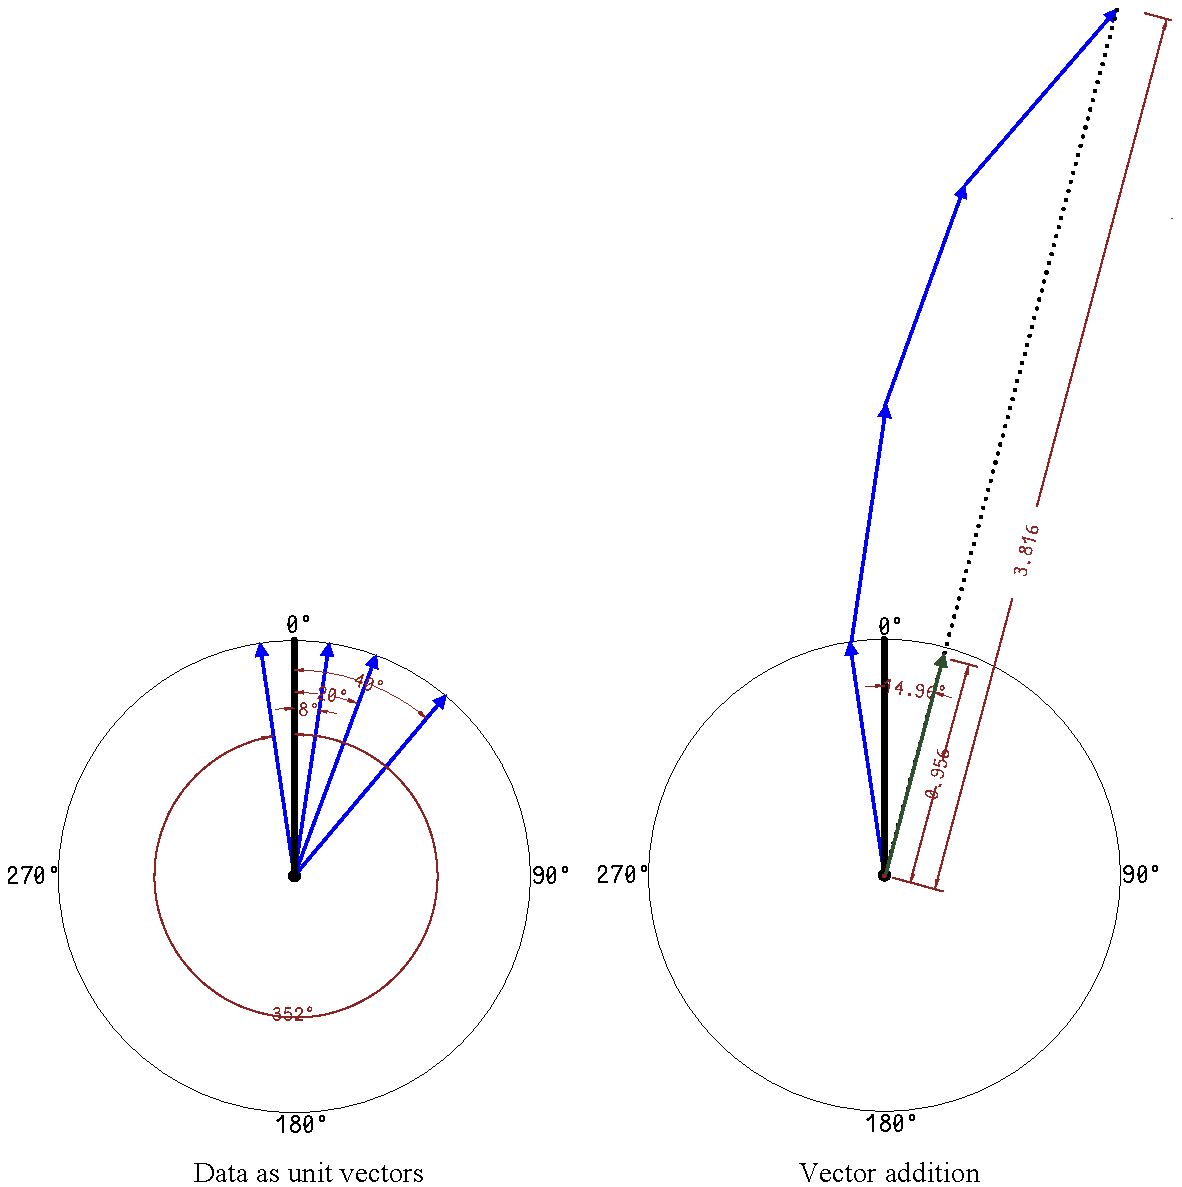
\includegraphics[width=0.7\textwidth]{Graphics/CircularMean}
\end{figure}


The data are plotted as unit vectors from the centre of a unit circle, with the angle identifying the direction of the vector (see fig. \ref{fig:CircMean}). The mean vector is then determined by vector addition of the data vectors.
\begin{eqnarray}
 \nonumber % Remove numbering (before each equation)
  C_p &=& \sum_{i = 1}^n{\cos(p \theta_i)} \\
 \nonumber
  S_p &=& \sum_{i = 1}^n{\sin(p \theta_i)} \\
 \nonumber
  R_p &=& \sqrt{C^2_p + S^2_p}, \quad [0\ldots n] \\
 \nonumber
 \bar{R}_p &=& R_p / n, \quad [0\ldots 1] \\
 \nonumber
  \bar{\theta}_p &=& \sin^{-1}(S_p/R_p) = \cos^{-1}(C_p/R_p) = \left\{
     \begin{array}{lr}
        \cos^{-1}(C_p/R_p) = \cos^{-1}(0) = \pi/2 &  C_p = 0          \\
        \tan^{-1}(S_p/C_p) + \pi                  &  C_p < 0          \\
        \tan^{-1}(S_p/C_p)                        &  S_p > 0, C_p > 0 \\
        \tan^{-1}(S_p/C_p) + 2\pi                 &  S_p < 0, C_p > 0
     \end{array}
   \right.
\end{eqnarray}
where \skalar{\bar{\theta}_p} is the mean vector direction and \skalar{\bar{R}_p} is the resultant length with respect to a positive whole number \skalar{p}. For the simple mean, \( p = 1 \), but higher values are required for some of the following. The sample statistics \skalar{\bar{\theta}_1} and \skalar{\bar{R}_1} (usually written \skalar{\bar{\theta}, \bar{R}}) estimate the population parameters \skalar{\mu} and \skalar{\rho}.

\begin{lstlisting}[caption=Arithmetic mean of circular data]
  FUNCTION MeanVector (TransformedData : VectorTyp; p : word) : ComplexTyp;

  VAR C, S, R, theta, Datum : float;
      n, i                  : WORD;

  BEGIN
     n  := VectorLength(TransformedData);
     C := 0;
     S := 0;
     FOR i := 1 TO n DO
       BEGIN
         Datum := GetVectorElement(TransformedData, i);
         C := C + Cos(p * Datum);
         S := S + Sin(p * Datum);
       END;
    R := Sqrt(C*C + S*S) / n;
    CASE signum(C) OF
      0 : theta := Const_pi / 2;    // arccos(C/R) = arccos(0)
     -1 : theta := ArcTan(S/C) + Const_pi;
      1 : CASE signum(S) OF
            1 :  theta := ArcTan(S/C);
           -1 :  theta := ArcTan(S/C) + Const_2pi;
            0 :  theta := 0;
      END;
    END;
    Result := ComplexInit(R, theta); // convert to complex number
  END;
\end{lstlisting}

\subsection{Spread}

The sample circular variance \skalar{V} and the sample circular standard deviation \skalar{v}  are calculated as follows:
\begin{eqnarray}
  V      &=& 1 - \bar{R}_1, \quad [0\ldots 1] \\
  v      &=& \sqrt{-2\ln(1-V)} = \sqrt{-2\ln(\bar{R}_1)}, \quad [0\ldots \infty]
\end{eqnarray}

\begin{lstlisting}[caption=Circular variance and standard deviation]
  FUNCTION CircularVariance (R : float) : float;

  BEGIN
    Result := 1 - R;
  END;

  FUNCTION CircularStandardDeviation (R : float) : float;

  BEGIN
    Result := sqrt(-2 * ln(R));
  END;
\end{lstlisting}

The maximum likelihood estimator for the parameter \skalar{\kappa} of the \Name{von Mieses} distribution is given by the approximation
\begin{equation}
  \hat{\kappa} = \left\{
          \begin{array}{l@{\;}l}
             2 \bar{R} + \bar{R}^3 + \frac{5 \bar{R}^5}{6}  & \quad \forall\ \bar{R} < 0.53 \\
             -0.4 + 1.39 \bar{R} + \frac{0.43}{1-\bar{R}}   & \quad \forall\ \bar{R} \in [0.53\ldots 0.85[\\
             \frac{1}{\bar{R}^3 - 4 \bar{R}^2 + 3 \bar{R}}  & \quad \forall\ \bar{R} \geq 0.85
          \end{array}
        \right.
\end{equation}
which for \( n \leq 15 \) needs a small sample correction
\begin{equation}
  \hat{\kappa}_c = \left\{
          \begin{array}{l@{\;}l}
             \max((\hat{\kappa} - 2/(n\hat{\kappa})), 0) & \quad \forall\ \hat{\kappa} < 2 \\
             (n-1)^3 \frac{\hat{\kappa}}{n^3 + n}        & \quad \forall\ \hat{\kappa} \geq 2
          \end{array}
        \right.
\end{equation}

\begin{lstlisting}[caption=Maximum likelihood estimator of \skalar{\kappa}]
  FUNCTION Kappa (R : float; n : WORD) : float;

  VAR k : float;

  BEGIN
    IF R < 0.53
      THEN
        k := 2*R + R*R*R + 5*pot(R, 5)/6
      ELSE
        IF R < 0.85
          THEN k := -0.4 + 1.39*R + 0.43/(1-R)
          ELSE k := 1 / (R*R*R - 4*R*R + 3*R);
    IF n <= 15  // small sample correction
      THEN
        IF k < 2
          THEN k := max((k - 2/(n*k)), 0)
          ELSE k := pot(Pred(n), 3) * k / (n*n*n + n);
    Result := k;
  END;
\end{lstlisting}

The median direction of a circular sample is the diameter of the circle that divides the data into two groups of equal size. However, we can use the median function for linear data only if all data are on the same side of the \texttt{0}-point.

\begin{lstlisting}[caption=Median of circular data]
  FUNCTION MedianDirection (TransformedData : VectorTyp) : float;

  BEGIN
    Result := Median(TransformedData);
  END;
\end{lstlisting}

\subsection{Higher moments}

The \skalar{p}th trigonometric moment (centred, that is, relative to the mean direction) is calculated by
\begin{equation}
  \mu_p = \frac{1}{n} \sum_{i=1}^n(\cos(p (\theta_i - \bar{\theta}))) + \imath \frac{1}{n} \sum_{i=1}^n(sin(p (\theta_i - \bar{\theta})))
\end{equation}

\begin{lstlisting}[caption=p-th trigonometric moment]
  FUNCTION TrigonometricMoment (Data : VectorTyp; MeanAngle : float; p : WORD) : ComplexTyp;

  VAR n, i : WORD;
      SumCos, SumSin, x : float;

  BEGIN
    n := VectorLength(Data);
    SumCos := 0;
    SumSin := 0;
    FOR i := 1 TO n DO
      BEGIN
        x := GetVectorElement(Data, i);
        SumSin := SumSin + Sin(p * (x - MeanAngle));
        SumCos := SumCos + Cos(p * (x - MeanAngle));
      END;
    Result := ComplexInit(SumCos/n, SumSin/n);
  END;
\end{lstlisting}

From these moments, we can calculate the \skalar{p}-th centred mean vector just like we did for the mean vector above:
\begin{lstlisting}[caption=p-th centered mean]
  function CenteredMean(Moment : ComplexTyp) : ComplexTyp;

  var S, C, R, theta : float;

  BEGIN
    C := Re(Moment);
    S := Im(Moment);
    R := sqrt(C*C + S*S);
    CASE signum(C) OF
      0 : theta := Const_pi / 2;    // arccos(C/R) = arccos(0)
     -1 : theta := ArcTan(S/C) + Const_pi;
      1 : CASE signum(S) OF
            1 :  theta := ArcTan(S/C);
           -1 :  theta := ArcTan(S/C) + Const_2pi;
            0 :  theta := 0;
      END;
    END;
    Result := ComplexInit(R, theta); // convert to complex number
  END;
\end{lstlisting}

From the first and second trigonometric moments \skalar{m_1, m_2} we calculate the circular dispersion as \( \delta = \frac{1 - \mu_2}{2 \mu_1^2} \)

\begin{lstlisting}[caption=Circular dispersion]
  FUNCTION CircularDispersion (TransformedData : VectorTyp; Mean : ComplexTyp) : float;

  var n, i         : word;
      R, theta, m2 : float;

  BEGIN
    n := VectorLength(TransformedData);
    theta := Im(Mean);
    m1 := Re(TrigonometricMoment(TransformedData, theta, 1));
    m2 := Re(TrigonometricMoment(TransformedData, theta, 2));
   Result := (1 - m2) / (2 * m1 * m1);
  END;
\end{lstlisting}

\subsubsection{Skew}

Skew can be calculated either from the original (\skalar{s}) or from the centred data (\skalar{s_0})
\begin{eqnarray}
  s   &=& \frac{1}{n} \sum_{i=1}^n sin(2 (\theta_i - \bar{\theta})) \\
  s_0 &=& \frac{R_2 \sin(\theta_2 - 2 \theta)}{1 - R}
\end{eqnarray}
A value close to \num{0} indicates a symmetrical distribution around the mean direction.

\begin{lstlisting}[caption=Circular skew]
  FUNCTION CircularSkew (TransformedData : VectorTyp; Mean : ComplexTyp) : float;

  VAR n, i          : WORD;
      theta, SumSin : float;

  BEGIN
    n := VectorLength(TransformedData);
    theta := Im(Mean); // mean angle
    SumSin := 0.0;
    FOR i := 1 TO n DO
      SumSin := SumSin + sin(2 * (GetVectorElement(TransformedData, i) - theta));
    Result := SumSin / n;
  END;


  FUNCTION CenteredCircularSkew (Mean1, Mean2 : ComplexTyp) : float;

  VAR theta1, theta2, R1, R2 : float;

  BEGIN
    theta1 := Im(Mean1);
    R1 := Re(Mean1);
    theta2 := Im(Mean2);
    R2 := Re(Mean2);
    Result := pot(1-R1, 2/3);
    IF Result = 0
      THEN
        BEGIN
          CircleError := true;
          WriteLn('Error: Circular skew when resultant length is 1');
          EXIT;
        END;
    Result := R2 * sin(theta2 - 2*theta1) / Result;
  END;
\end{lstlisting}

\subsubsection{Kurtosis}

The circular kurtosis we also can calculate centred or non-centred
\begin{eqnarray}
  k   &=& \frac{1}{n} \sum_{i=1}^n cos(2 (\theta_i - \bar{\theta})) \\
  k_0 &=& \frac{R_2 \cos(\theta_2 - 2 \bar{\theta}) - R^4}{(1 - R)^2}
\end{eqnarray}
, a value close to \num{1} indicates a strongly peaked distribution. If the data come from a \Name{von Mieses} distribution, then \( k_0 = 0 \).

\begin{lstlisting}[caption=Circular kurtosis]
  FUNCTION CircularKurtosis (TransformedData : VectorTyp; Mean : ComplexTyp) : float;

  VAR n, i          : WORD;
      theta, SumCos : float;

  BEGIN
    n := VectorLength(TransformedData);
    theta := Im(Mean); // mean angle
    SumCos := 0.0;
    FOR i := 1 TO n DO
      SumCos := SumCos + cos(2 * (GetVectorElement(TransformedData, i) - theta));
    Result := SumCos / n;
  END;


  FUNCTION CenteredCircularKurtosis (Mean1, Mean2 : ComplexTyp) : float;

  VAR theta1, theta2, R1, R2 : float;

  BEGIN
    theta1 := Im(Mean1);
    R1 := Re(Mean1);
    theta2 := Im(Mean2);
    R2 := Re(Mean2);
    Result := sqr(1-R1);
    IF Result = 0
      THEN
        BEGIN
          CircleError := true;
          WriteLn('Error: Circular kurtosis when resultant length is 1');
          EXIT;
        END;
    Result := (R2 * cos(theta2 - 2*theta1) - pot(R1, 4)) / Result;
  END;
\end{lstlisting}

\subsection{Confidence interval for mean direction}

If the allowable error is \skalar{\delta}, then the confidence interval \( d(1 - \delta) \) is computed by
\begin{equation}
  d = \left\{
          \begin{array}{l@{\;}l}
             \arccos\left[\frac{\sqrt{\frac{2 n (2 {(\bar{R} n)^2 - n \chi^2_{\delta,1}})}{4 n - \chi^2_{\delta,1}}}}{\bar{R} n} \right]    & \quad \forall\ \bar{R} \leq 0.9 \wedge \bar{R} > \sqrt{\frac{\chi^2_{\delta,1}}{2n}} \\
              & \\
             \arccos\left[\frac{\sqrt{n - {n^2 - (\bar{R} n)^2} \exp(\frac{\chi^2_{\delta,1}}{n})}}{\bar{R} * n} \right]    & \quad \forall\ \bar{R} > 0.9 \\
          \end{array}
        \right.
\end{equation}
The confidence interval is then \( \bar{\theta} \pm d \).

\begin{lstlisting}[caption=Confidence interval of circular mean]
  FUNCTION ConfidenceInterval (R, delta : float; n : WORD) : float;

  VAR Rn, chi : float;
      c       : CHAR;

  BEGIN
    Rn := R * n;
    chi := SignificanceLimit_Chi2(delta, 1);
    IF R > 0.9
      THEN
        Result := arccos(Sqrt(n - (n*n - Rn*Rn) * Exp(chi/n))/Rn)
      ELSE IF R > Sqrt(chi/(2*n))
             THEN
               Result := arccos(Sqrt((2 * n * (2*Rn*Rn - n*chi)) / (4*n - chi))/Rn)
             ELSE
               BEGIN
                 c := WriteErrorMessage('Confidence interval of mean angle: vector length to small');
                 CircleError := TRUE;
                 EXIT;
               END;
  END;
\end{lstlisting}

\section{Pseudo-random variables }

\begin{figure}
 \caption{\capstart Random variables of different distributions. \emph{Right}: Uniformly distributed. \emph{Left + middle}: \Name{von Mieses} distributed with different mean direction \skalar{\bar{\theta}} and spread \skalar{\kappa}.}
 \label{fig:CircRand}
 \centering
 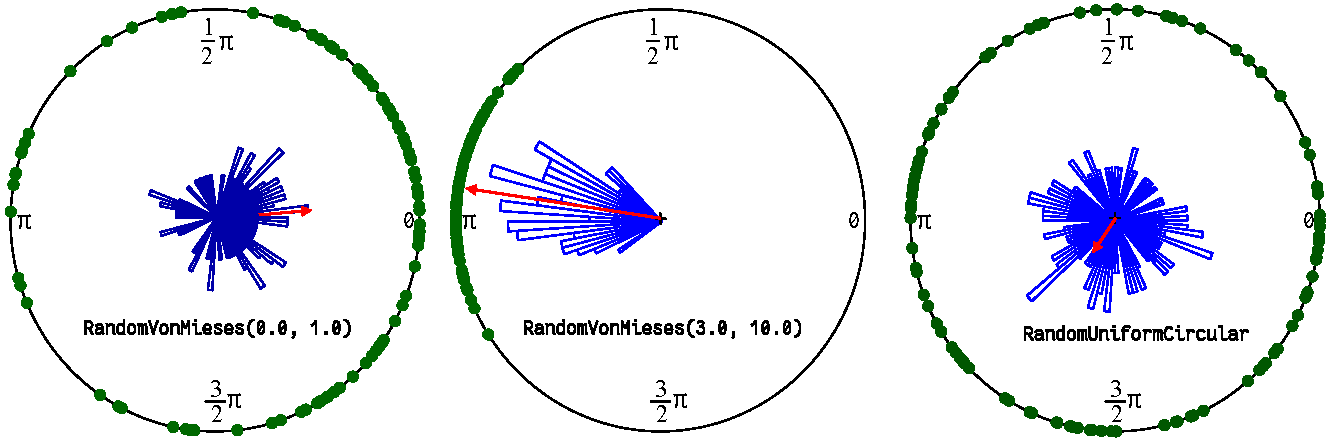
\includegraphics[width=\textwidth]{Graphics/c1-mean}
\end{figure}


The following routine returns a \Name{von Mieses}-distributed pseudo-random number, the algorithm is described in \parencite{Bar-95} (see fig. \ref{fig:CircRand}).

\begin{lstlisting}[caption=von Mieses distributed random number]
  FUNCTION RandomVonMieses(mu, kappa : float) : float;

  VAR s, u1, u2, theta : float;

  BEGIN
    IF kappa > 1.3
      THEN s := 1/Sqrt(kappa)
      ELSE s := Const_pi * Exp(-kappa);
    REPEAT
      u1 := Random;
      u2 := Random;
      theta := s*(2*u2 - 1) / u1;    // generate prospective value
      IF Abs(theta) < Const_pi       // rejection pre-TEST
        THEN
          IF ((kappa*theta*theta) < (4 - 4*u1))  // acceptance pre-TEST
            THEN
              BEGIN
                Result := ModuloTwoPi(theta + mu);
                EXIT;
              END
            ELSE
              IF ((kappa*Cos(theta)) > (2*Ln(u1) + kappa))
                THEN
                  BEGIN
                    Result := ModuloTwoPi(theta + mu);
                    EXIT;
                  END
               ELSE  // IF < THEN TRY again
        ELSE // IF > THEN TRY again
    UNTIL FALSE;
  END;
\end{lstlisting}

Random numbers uniformly distributed around the circle are a useful \texttt{0}-model:

\begin{lstlisting}[caption=Random data uniformly distributed over a circle]
  FUNCTION RandomUniformCircular : float;

  BEGIN
    Result := Random * Const_2pi;
  END;
\end{lstlisting}

\section{Statistical tests for a single circular data set}

\subsection{Do samples have a preferred direction}

These procedures test \textbf{\skalar{H_0}: The data are uniformly distributed} against \textbf{\skalar{H_1}: There is a preferred direction}.

\subsubsection{The \Name{Rayleigh}-test}

From the discussion above it is clear that the closer the data cluster toward a main direction, the larger the length of the mean vector becomes. Thus, \textbf{\skalar{H_0}} could also be phrased as \( \bar{R} = 0 \) and \textbf{\skalar{H_1}} as \( \bar{R} > 0 \). For \( n > 10 \) and \Name{von Mieses}-distributed data the probability for \textbf{\skalar{H_0}} becomes:
\begin{equation}
  P_0 \approx\ \exp \left[\sqrt{1 + 4n + 4(n^2 - R^2)} - (1 + 2n))\right]
\end{equation}
This test is suitable only for unimodal data. Note that in the formula \skalar{R} is used, not \( \bar{R} \). For consistency, the following function accepts \( \bar{R} \), however.

\begin{lstlisting}[caption=Rayleigh-test]
  FUNCTION Rayleigh (MeanVectorLength : float; n : WORD) : float;

  VAR c : CHAR;
      x : float;

  BEGIN
    IF (n < 10)
      THEN
        BEGIN
          c := WriteErrorMessage('Rayleigh test with less than 10 data points');
          CircleError := TRUE;
          EXIT;
        END;
    x := MeanVectorLength * n; // convert TO unscaled
    Result := Exp(Sqrt(1 + 4*n + 4*(n*n - x*x)) - (1 + 2*n));
  END;
\end{lstlisting}


\subsubsection{The \Foreign{omnibus} test of \Name{Hodges-Ajne}}

If the data are plotted on a circle, and a diameter is drawn through that circle, some data will be on one, the others on the other side of that diameter. The diameter line is then rotated until the number of data points on the ``wrong'' side (\skalar{m}) becomes minimal. Actually (at least in unimodal distributions), the diameter that produces minimal \skalar{m} must be the one at right angle to the mean vector. \skalar{m} will be the smaller the more directional the data are. This test is non-parametric and does not require the data to be \Name{von Mieses} distributed (hence ``\Foreign{omnibus}'' = Lat. ``for all'', here: irrespective of a data model). The probability, to observe a \skalar{m} this small for randomly distributed data becomes
\begin{equation}
  P_0 = \frac{1}{2^{n-1}}\ (n - 2m)\ \binom{n}{m}
\end{equation}
As a non-parametric test, this test is less powerful than the \Name{Rayleigh}-test.

\begin{lstlisting}[caption=Omnibus-test]
  FUNCTION HodgesAjne (TransformedData : VectorTyp; MeanAngle : float) : float;

  VAR StartAngle, StopAngle, x : float;
      i, m1, m2, n             : WORD;

  BEGIN
    StartAngle := ModuloTwoPi(MeanAngle - Nintey);
    StopAngle := ModuloTwoPi(MeanAngle + Nintey);
    IF StartAngle > StopAngle
      THEN
        BEGIN // exchange start- and stop angle
          x := StartAngle;
          StartAngle := StopAngle;
          StopAngle := x;
        END;
    n := VectorLength(TransformedData);
    m1 := 0;
    m2 := 0;
    FOR i := 1 TO n DO
      BEGIN
        x := GetVectorElement(TransformedData, i);
        IF (x >= StartAngle) AND (x <= StopAngle)
          THEN INC(m1)  // count # OF data points on either side of the diameter
          ELSE INC(m2);
      END;
    IF (m1 > m2) THEN m1 := m2; // peak on the other side of diameter
    Result := 1/pot(2, Pred(n)) * (n - 2*m1) * BinomialCoef(n, m1);
  END;
\end{lstlisting}


\subsubsection{The \skalar{\chi^2}-test}

Input parameters are the data vector (transformed to \( [0\ldots 2\pi] \)), the direction of the mean vector, and the number of sectors. Output data are the \skalar{\chi^2} and the degrees of freedom.

\begin{lstlisting}[caption=\skalar{\chi^2}-test for homogeneous distribution]
  PROCEDURE ChiSqrTest (Data : VectorTyp; Direction : float; Sectors : WORD;
                        VAR ChiSqr : float; VAR dgf : WORD);

  VAR i, j, Counter, n, max : WORD;
      Expected, Angle,
      StartAngle,
      Start, Finish, x      : float;
      Dummy                 : CHAR;
      ErrorStr, s           : STRING;

  BEGIN
    n := VectorLength(Data);
    IF n < 8
      THEN
        BEGIN
          CircleError := TRUE;
          Dummy := WriteErrorMessage('Not enough data for ChiSqr-test (> 8 required)');
          EXIT;
        END;
    max := n DIV 4;
    IF max > 250 THEN max := 250;
    Expected := n / Sectors;
    IF Expected < 4
      THEN
        BEGIN
          CircleError := TRUE;
          Str(n:4, ErrorStr);
          Str(max:4, s);
          ErrorStr := ErrorStr + 'Data points allow at most ' + s + ' sectors';
          Dummy := WriteErrorMessage(ErrorStr);
          EXIT;
        END;
    ChiSqr := 0.0;
    Angle := Const_2pi / Sectors;
    StartAngle := Direction - 0.5 * Angle;
    dgf := Pred(Sectors);
    FOR i := 1 TO Sectors DO
      BEGIN
        Start := StartAngle + Pred(i) * Angle;
        Finish := Start + Angle;
        Counter := 0;
        FOR j := 1 TO n DO
          BEGIN
            x := GetVectorElement(Data, j);
            IF (Start <= Const_2pi) AND (Finish <= Const_2pi)
              THEN
                IF (x > Start) AND (x < Finish)
                  THEN INC(Counter)
                  ELSE // outside SECTOR
              ELSE
                IF (Start < Const_2pi) AND (Finish > Const_2pi)
                  THEN
                    IF ((x > Start) AND (x < Const_2pi)) OR (x < ModuloTwoPi(Finish))
                      THEN INC(Counter)
                      ELSE
                  ELSE
                    IF (x > ModuloTwoPi(Start)) AND (x < ModuloTwoPi(Finish))
                      THEN INC(Counter);
            END; // FOR j
         ChiSqr := ChiSqr + Sqr(Counter - Expected) / Expected;
      END;  // FOR i
  END;
\end{lstlisting}

\subsubsection{\skalar{V}-test for uniformity against a suspected direction}

Sometimes one can specify an expected value for the mean vector direction \emph{before} an experiment is undertaken. Then a test for randomness needs not exclude all other possible models, hence the ``\skalar{V}-test'' is more efficient \parencite{Gre-55}. Thus, \textbf{\skalar{H_0}: The data are homogeneously distributed} against \textbf{\skalar{H_1}: The data cluster around a hypothetical direction \skalar{\theta_A}}. Note that the test applies only to randomness, it is not useful to decide whether the mean direction coincides with the expected direction. The test statistics is
\begin{equation}
  V = \sqrt{\frac{2}{n}}\ R\ cos(\bar{\theta} - \theta_A)
\end{equation}
However, if the test fails to reach significance, it is unclear whether the data are uniformly distributed or the expected value was wrong.

\begin{lstlisting}[caption=V-test for random distribution against suspected direction]
  FUNCTION HomewardComponent (n : WORD; Mean : ComplexTyp; Expected : float) : float;

  VAR Length, Phi, v : float;

  BEGIN
    Polar(Mean, Length, Phi);
    Phi := ModuloTwoPi(Phi);
    v := Length * Cos(Phi - Expected);
    Result := Sqrt(2*n) * v;
  END;
\end{lstlisting}

\subsubsection{\Name{Rao}'s spacing test}

If circular data are randomly distributed, then their distance from each other should be roughly \( \lambda = \frac{360}{n} \) \parencite{Rao-76}. If the data are clustered, some distances should be significantly larger than others. The test statistics becomes:
\begin{equation}
  U = \frac{1}{2} \sum_{i=1}^{n-1}{|(\theta_{i+1} - \theta_i) - \lambda|}
\end{equation}
\Name{Rao}'s test can be used for uni- and multimodal data, the critical values of \skalar{U} are tabulated in \parencite{Rus-95}.

\begin{lstlisting}[caption=\Name{Rao}'s test]
  FUNCTION Rao (TransformedData : VectorTyp) : float;

  VAR T, SumT, Expected : float;
      i, n              : WORD;

  BEGIN
    n := VectorLength(TransformedData);
    Expected := Const_2pi / n;
    SumT := 0;
    FOR i := 2 TO n DO
      BEGIN
        T := GetVectorElement(TransformedData, i) - GetVectorElement(TransformedData, Pred(i));
        SumT := SumT + Abs(T - Expected);
      END;
    T := Const_2pi + GetVectorElement(TransformedData, 1) - GetVectorElement(TransformedData, n);
    SumT := SumT + Abs(T - Expected);
    Rao := 0.5 * SumT;
  END;
\end{lstlisting}

\subsubsection{\Name{Kuipers}'s test against a suspected distribution}

\Name{Kuipers}'s test compares a given distribution of data with a theoretical model. The data matrix contains in the first column the angle, in the second the measured cumulative frequency and in the third the theoretical cumulative frequency (both in the range \( [0\ldots 1] \)). Returned are \skalar{V_n} and \skalar{K}.

\begin{lstlisting}[caption=\Name{Kuipers}'s test]
  PROCEDURE Kuipers (Data : MatrixTyp; VAR K, U : float);

  VAR DPlus, DMinus, c, vSqr, cvn, vSum,
      Diff, Diff1, Diff2, Vn, vMean, x    : float;
      n, i                                : WORD;
      xVector, yVector,
      bVector                             : VectorTyp;

  BEGIN
    n := MatrixRows(Data);
    GetColumn(Data, 1, xVector);
    GetColumn(Data, 2, yVector);
    GetColumn(Data, 3, bVector);
    vSum := NeumaierSum(bVector);
    vMean := vSum / n;
    DPlus := 0.0;
    DMinus := 0.0;
    vSqr := 0.0;
    cvn := 0.0;
    FOR i := 1 TO n DO
      BEGIN
        x := GetVectorElement(bVector, i);
        Diff  := GetVectorElement(yVector, i) - x;
        Diff1 := GetVectorElement(yVector, Pred(i)) - x;
        Diff2 := GetVectorElement(yVector, Succ(i)) - x;
        IF Diff  > DPlus THEN DPlus := Diff;
        IF Diff1 > DPlus THEN DPlus := Diff1;
        IF Diff  < DMinus THEN DMinus := Diff;
        IF Diff1 < DMinus THEN DMinus := Diff1;
        c := Pred(2 * i);
        cvn := cvn + c * GetVectorElement(bVector, i) / n;
        vSqr := vSqr + Sqr(GetVectorElement(bVector, i));
      END;  // FOR
    Vn := (DPlus + Abs(DMinus)) * Sqrt(n);
    K := Vn;
    U := vSqr - cvn + n * (1/3 - Sqr(vMean - 0.5));
    DestroyVector(xVector);
    DestroyVector(yVector);
    DestroyVector(bVector);
  END;
\end{lstlisting}

The following routine creates the table with cumulative frequencies needed by \Name{Kuipers}'s test.

\begin{lstlisting}[caption=Create frequency table]
  procedure CalculateCumulativeFrequencies (Data : VectorTyp; FullCircle : float;
                                        var Result : MatrixTyp);

  var i, n : word;
      Wert : float;
      D    : VectorTyp;

  begin
    n := VectorLength(Data);
    CopyVector(Data, D);
    ShellSort(D);
    for i := 1 to n do
     begin
       Wert := GetVectorElement(D, i);
       SetMatrixElement(Result, i, 1, Wert);
       SetMatrixElement(Result, i, 2, i/n);
       SetMatrixElement(Result, i, 3, Wert/FullCircle);
     end;
    DestroyVector(D);
  end;
\end{lstlisting}

\subsubsection{One sample \skalar{t}-test}

This test is used to test \textbf{\skalar{H_0}: The population mean angle \skalar{\bar{\theta}} is equal to \skalar{\theta_0}} against \textbf{\skalar{H_1}: The population mean angle \skalar{\bar{\theta}} is different from \skalar{\theta_0}}. This test is performed by checking if \( \theta_0 \in \bar{\theta} \pm d(1-\delta) \), that is, \skalar{\theta_0} is between the upper and lower confidence limits.

\begin{lstlisting}[caption=One-sample \skalar{t}-test]
  FUNCTION OneSample (MeanAngle, R, delta, TestAngle : float; n : WORD) : BOOLEAN;

  VAR x : float;

  BEGIN
    x := ConfidenceInterval(R, delta, n);
    Result := (TestAngle > (MeanAngle - delta)) AND (TestAngle < (MeanAngle + delta));
  END;
\end{lstlisting}

\subsubsection{Binomial test for median angle}

This is a non-parametric test with a similar purpose as the one-sample test, however, it is based on the median rather than mean angle. \textbf{\skalar{H_0}: The population median angle \skalar{\breve{\theta}} is equal to \skalar{\theta_0}}. If \textbf{\skalar{H_0}} holds, then \skalar{\theta_0} should divide the data set into two nearly identical halfs, the number of data on either side should fall under the binomial distribution \( k = B(n, 0.5) \).

\subsection{Symmetry around \skalar{\breve{\theta}}}

If the data set is symmetrical around \skalar{\breve{\theta}}, then the median circular distance of the data points from the median \skalar{\breve{\theta}} should be zero. This can be tested by a \Name{Wilcoxon} signed rank test.

\subsection{Grouped data}

The data matrix contains circular data in grouped form: first column the middle of the range of angles, the second column the counts. The angles must be distributed across the circle evenly.

\begin{lstlisting}[caption=Mean direction of grouped data]
  FUNCTION MeanVectorGrouped (Transformed : MatrixTyp; Difference : float) : ComplexTyp;

  VAR Total, n, i, j : WORD;
      x, y, z,
      Length, Angle  : float;
      Coord          : ComplexTyp;

  BEGIN
      n := MatrixRows(Transformed);
      Total := 0;
      x := 0.0;
      y := 0.0;
      FOR i := 1 TO n DO
        BEGIN
          j := Round(GetMatrixElement(Transformed, i, 2));
          z := GetMatrixElement(Transformed, i, 1);
          Total := Total + j;
          x := x + j * Cos(z);
          y := y + j * Sin(z);
        END;
      x := x / Total;
      y := y / Total;
      Coord := ComplexInit(x, y);      // Re, Im
      Polar(Coord, Length, Angle);     // polar coordinates
      z := Difference / 2;
      z := z / Sin(z);
      Length := Length * z;            // correct quantisation error
      Result := Rect(Length, Angle);   // back TO cartesian coordinates }
  END;
\end{lstlisting}

\section{Multi-sample tests}

\subsection{\Name{Watson-Williams}-test: two vectors with circular data}

This test is the circular equivalent of the two-sample \skalar{t}-test for linear data, it assesses the question whether \skalar{s} data sets come from distributions with the same mean angle \parencite{wat-56, Ste-69}.
\begin{equation}
  F = K \frac{(n - s)(\sum_{j=1}^s(R_j - R))}{(s-1) (n - \sum_{j=1}^s(R_j))}, \quad K = 1 + \frac{3}{8\kappa}
\end{equation}
where \skalar{R_j} is the separate mean vector length for the \skalar{j}th group. \skalar{\kappa} is an estimator for the dispersion of the \Name{von Mieses} distribution. The resulting test statistics is compared with the critical value of \skalar{F_{\delta, 1, n-2}}.

The test is relatively robust against violations of the \Name{von Mieses} distribution, as long as all groups have at least \num{5} members.

\begin{lstlisting}[caption=Watson-Williams test]
  PROCEDURE WatsonWilliams (TransformedData1, TransformedData2 : VectorTyp);

  VAR Transformed3                                   : VectorTyp;
      Mean1, Mean2, Mean3                            : ComplexTyp;
      Length1, Length2, Length3, Phi1, Phi2, Phi3,
      x, r, g, F, P0                                 : float;
      i, n1, n2, n3, nMean                           : WORD;
      hst                                            : STRING;

   BEGIN
    n1 := VectorLength(TransformedData1);
    n2 := VectorLength(TransformedData2);
    n3 := n1 + n2;
    CreateVector(Transformed3, n3, 0.0);
    FOR i := 1 TO n1 DO
      SetVectorElement(Transformed3, i, GetVectorElement(TransformedData1, i));
    FOR i := 1 TO n2 DO
      SetVectorElement(Transformed3, n1+i, GetVectorElement(TransformedData2, i));
    Mean1 := MeanVector(TransformedData1);
    Polar(Mean1, Length1, Phi1);
    Phi1 := ModuloTwoPi(Phi1);
    Mean2 := MeanVector(TransformedData2);
    Polar(Mean2, Length2, Phi2);
    Phi2 := ModuloTwoPi(Phi2);
    Mean3 := MeanVector(Transformed3);
    Polar(Mean3, Length3, Phi3);
    Phi3 := ModuloTwoPi(Phi3);
    r := (Length1 + Length2) / 2;
    nMean := (n1 + n2) DIV 2;
    g := 1 + 3 / (8 * Kappa(r, nMean));
    F := g * (Length1 + Length2 - Length3) / (n3 - (Length1 + Length2));
    P0 := Integral_F(F, 1, n3-2);
    Writeln('F = ', FloatStr(F, ValidFigures), ', f1 = 1, f2 = ', n3-2:4,
            ' => P0 = ' + FloatStr(P0, ValidFigures));
    DestroyVector(Transformed3);
  END;
\end{lstlisting}

\subsection{Circular \Name{Kruskal-Wallis}-test for equal median}

Non-parametric test for \textbf{\skalar{H_0}:  \( \breve{\theta}_1 = \breve{\theta}_2 = \ldots = \breve{\theta}_s \)} against \textbf{\skalar{H_1}: At least one of the data set has a different median}. The test works by first calculating the overall median of the combined data set. Then for each group \skalar{i} we calculate \skalar{m_i}, the number of samples \skalar{\theta_j^i} (\skalar{j}th sample in the \skalar{i}th group) where the distance \( d(\theta_j^i, \breve{\theta}) \) is negative. Then the test statistics
\begin{equation}
  x = \frac{N^2}{M (N-M)}\sum_{i=1}^s\frac{m_i^2}{n_i} - \frac{N M}{N - M}
\end{equation}
(\skalar{M, N} total over all groups, \skalar{m_i, n_i} within the \skalar{i}th group) is compared with the upper \skalar{1-\delta}th percentile of the \skalar{\chi^2(\delta, s-1)} distribution. The test is valid only if all \( n_i > 10 \).

\begin{lstlisting}[caption=Kruskal-Wallis test]
  FUNCTION KruskalWallis (TransformedData1, TransformedData2 : VectorTyp) : float;

  VAR Data3                            : VectorTyp;
      Median3, x, xmin, xmax, P           : float;
      i, n1, n2, n3, m1, m2, m                          : WORD;
      c                                              : CHAR;

  BEGIN
    n1 := VectorLength(TransformedData1);
    n2 := VectorLength(TransformedData2);
    n3 := n1 + n2;
    IF (n1 <= 10) OR (n2 <= 10)
      THEN
        BEGIN
          c := WriteErrorMessage('Circular Kruskal-Wallis test: n > 10 required for all groups');
          CircleError := TRUE;
          EXIT;
        END;
    CreateVector(Data3, n3, 0.0);
    FOR i := 1 TO n1 DO
      SetVectorElement(Data3, i, GetVectorElement(TransformedData1, i));
    FOR i := 1 TO n2 DO
      SetVectorElement(Data3, n1+i, GetVectorElement(TransformedData2, i));
    ShellSort(Data3);
    Median3 := MedianDirection(Data3);
    xmin := ModuloTwoPi(Median3 + Nintey);
    xmax := ModuloTwoPi(Median3 - Nintey);
    m1 := 0;
    FOR i := 1 TO n1 DO
      BEGIN
        x := GetVectorElement(TransformedData1, i);
        IF (x > xmin) AND (x < xmax) THEN INC(m1);
      END;
    m2 := 0;
    FOR i := 1 TO n2 DO
      BEGIN
        x := GetVectorElement(TransformedData2, i);
        IF (x > xmin) AND (x < xmax) THEN INC(m2);
      END;
    m := m1 + m2;
    P := n3*n3 / (m * (n3 - m)) * (m1*m1/n1 + m2*m2/n2) - n3 * m / (n3 - m);
    Result := IntegralChi(P, 1);
    Writeln('Chi^2 = ', FloatStr(P, ValidFigures), ' with 1 degrees of freedom, P0 = ',
            FloatStr(x, ValidFigures));
    DestroyVector(Data3);
  END;
\end{lstlisting}

\subsection{Difference between two vectors}

Calculates the cumulative frequencies of both data vectors and calculates \Name{Kuiper}'s \skalar{V} und \Name{Whatson}'s \skalar{U^2}. The data vectors must be sorted.

\begin{lstlisting}[caption=Difference between two vectors]
  PROCEDURE Difference (Data1, Data2 : VectorTyp; VAR KuipersV, WatsonsUSqr : float);

  TYPE ListenRecTyp = RECORD
                        Angle, k1, k2 : float;
                      END;

  VAR n1, n2, Cumulative1, Cumulative2                  : WORD;
      Diff, Dif, DifSqr, DifPos, DifNeg, Angle1, Angle2 : float;
      ListenRec                                         : ListenRecTyp;
      Liste                                             : FiFo;

  BEGIN
    n1 := VectorLength(Data1);
    n2 := VectorLength(Data2);
    ShellSort(Data1);
    ShellSort(Data2);
    Cumulative1 := 0;
    Cumulative2 := 0;
    InitFiFo(Liste);
    WHILE (Cumulative1 < n1) AND (Cumulative2 < n2) DO          { Data durchlaufen, }
      BEGIN                                                     { cumulative Frequenzen }
        Angle1 := GetVectorElement(Data1, Succ(Cumulative1));   { erzeugen und in FIFO  }
        Angle2 := GetVectorElement(Data2, Succ(Cumulative2));   { Liste speichern }
        IF Angle1 < Angle2
          THEN
           BEGIN
               INC(Cumulative1);
               ListenRec.Angle := Angle1;
           END
          ELSE
           BEGIN
               INC(Cumulative2);
               ListenRec.Angle := Angle2;
           END;
        ListenRec.k1 := 1.0 * Cumulative1 / n1;
        ListenRec.k2 := 1.0 * Cumulative2 / n2;
        Put(Liste, ListenRec, SizeOf(ListenRec));
      END; { while }
    WHILE (Cumulative1 < n1) DO                               { eventuell übrig gebliebene }
     BEGIN                                                    { Elemente aus 1. Datasatz  }
       INC(Cumulative1);                                      { bearbeiten }
       ListenRec.k1 := 1.0 * Cumulative1 / n1;
       ListenRec.k2 := 1.0 * Cumulative2 / n2;
       ListenRec.Angle := GetVectorElement(Data1, Cumulative1);
       Put(Liste, ListenRec, SizeOf(ListenRec));
     END;
    WHILE (Cumulative2 < n2) DO                               { dito für 2. Datasatz }
     BEGIN
       INC(Cumulative2);
       ListenRec.k1 := 1.0 * Cumulative1 / n1;
       ListenRec.k2 := 1.0 * Cumulative2 / n2;
       ListenRec.Angle := GetVectorElement(Data2, Cumulative2);
       Put(Liste, ListenRec, SizeOf(ListenRec));
     END;
    DifPos := 0.0;
    DifNeg := 0.0;
    Dif    := 0.0;
    DifSqr := 0.0;
    WHILE NOT EmptyFiFo(Liste) DO                             { Liste durchlaufen und }
      BEGIN                                                   { größte positive und   }
        Get(Liste, ListenRec, SizeOf(ListenRec));             { negative Difference suchen }
        Diff := ListenRec.k1 - ListenRec.K2;
        IF Diff > DifPos THEN DifPos := Diff;
        IF Diff < DifNeg THEN DifNeg := Diff;
        Dif := Dif + Diff;                                    { aufsummieren für Watson's Test }
        DifSqr := DifSqr + Sqr(Diff);
      END;
    KuipersV := n1 * n2 * (DifPos - DifNeg);
    WatsonsUSqr := n1 * n2 / Sqr(n1+n2) * (DifSqr - Sqr(Dif) / (n1+n2));
  END;
\end{lstlisting}

Under the condition that the data are \Name{von-Mises}-distributed, the following routine calculates the \skalar{F}-value for \textbf{\skalar{H_0}: \( \kappa_1 = \kappa_2 \)} against \textbf{\skalar{H_1}: \( \kappa_1 \neq \kappa_2 \)}. The probability of \skalar{H_0} is then obtained by integrating the \skalar{F}-distribution with \skalar{n_1, n_2} degrees of freedom. If \( F < 1 \), the integration has to be performed with \skalar{1/F} and exchanged degrees of freedom.

\begin{lstlisting}[caption=F-test]
  FUNCTION FTest (Data1, Data2 : VectorTyp) : float;

  VAR Mean1, Mean2                               : ComplexTyp;
      Angle1, Angle2, Length1, Length2, rMean    : float;
      n1, n2                                     : WORD;

  BEGIN
    n1 := VectorLength(Data1);
    Mean1 := MeanVector(Data1, 1);
    Polar(Mean1, Length1, Angle1);
    n2 := VectorLength(Data2);
    Mean2 := MeanVector(Data2, 1);
    Polar(Mean2, Length2, Angle2);
    Length1 := Length1 * n1;
    Length2 := Length2 * n2;
    rMean := (Length1 + Length2) / (n1 + n2);
    IF rMean < 0.7
      THEN
       BEGIN
         CH := WriteErrorMessage('Mean vectors to short, F-Test not applicable');
         CircleError := TRUE;
         EXIT;
       END;
    Result := Pred(n2) * (n1 - Length1) / (Pred(n1) * (n2 - Length2));
  END;
\end{lstlisting}

\Name{Wilcoxon}'s non-parametric test for \textbf{\skalar{H_0}: The data sets have the same standard deviation} vs. \textbf{\skalar{H_1}: The data sets have different standard deviations}. \texttt{Direction1} and \texttt{-2} contain either the mean direction of the data vectors, or a common homeward component. In the latter case, the test is for equal/unequal home-finding ability. The function returns the \Name{Wilcoxon-Mann-Whitney} \skalar{U}-value. All data must be in \( [0..2\pi] \).

\begin{lstlisting}[caption=Wilcoxon's non-parametric test for equal standard deviation]
  FUNCTION Wilcoxon (Data1, Data2 : VectorTyp; Direction1, Direction2 : float) : float;

  VAR U1, U2, x                       : float;
      n1, n2, Rank, i, j, Sum1, Sum2  : WORD;
      Diff1, Diff2                    : VectorTyp;

  BEGIN
    n1 := VectorLength(Data1);
    CreateVector(Diff1, n1, 0.0);
    FOR i := 1 TO n1 DO
     BEGIN
       x := Abs(GetVectorElement(Data1, i) - Direction1);
       IF x > Pi
         THEN SetVectorElement(Diff1, i, Const_2pi-x)
         ELSE SetVectorElement(Diff1, i, x);
     END;
    ShellSort(Diff1);
    n2 := VectorLength(Data2);
    CreateVector(Diff2, n2, 0.0);
    FOR i := 1 TO n2 DO
     BEGIN
       x := Abs(GetVectorElement(Data2, i) - Direction2);
       IF x > Pi
         THEN SetVectorElement(Diff2, i, Const_2pi-x)
         ELSE SetVectorElement(Diff2, i, x);
     END;
    ShellSort(Diff2);
    Rank := 1;
    j := 1;
    Sum1 := 0;
    Sum2 := 0;
    IF n1 < n2
      THEN
       BEGIN
         FOR i := 1 TO n1 DO
           BEGIN
             WHILE (GetVectorElement(Diff2, j) < GetVectorElement(Diff1, i)) DO
               BEGIN
                 INC(Sum2, Rank);
                 INC(Rank);
                 INC(j);
               END;
             INC(Sum1, Rank);
             INC(Rank);
           END;
         FOR i := j TO n2 DO
          BEGIN
            INC(Sum2, Rank);
            INC(Rank);
          END;
       END
      ELSE
       BEGIN
         FOR i := 1 TO n2 DO
           BEGIN
             WHILE (GetVectorElement(Diff1, j) < GetVectorElement(Diff2, i)) DO
               BEGIN
                 INC(Sum1, Rank);
                 INC(Rank);
                 INC(j);
               END;
             INC(Sum2, Rank);
             INC(Rank);
           END;
         FOR i := j TO n1 DO
          BEGIN
            INC(Sum1, Rank);
            INC(Rank);
          END;
       END;
    DestroyVector(Diff1);
    DestroyVector(Diff2);
    U1 := Sum1 - n1 * Succ(n1) / 2;
    U2 := Sum2 - n2 * Succ(n2) / 2;
    IF U1 < U2
      THEN Result := U1
      ELSE Result := U2;
  END;
\end{lstlisting}

\begin{lstlisting}[caption=]
  PROCEDURE DescribeBivariat (Data : MatrixTyp);

  VAR i, n1                                                     : WORD;
      SumX, SumY, a, b, c, d, r, SumXSqr, SumYSqr, SumXDevYDev,
      xSta, ySta, xMean, yMean, CoVariance, Correlation, Phi,
      Major, Minor, xMin, xMax, yMin, yMax                      : float;

  BEGIN
    SumX := 0.0;
    SumY := 0.0;
    SumXSqr := 0.0;
    SumYSqr := 0.0;
    SumXDevYDev := 0.0;
    n1 := MatrixRows(Data);
    xMin := MaxRealNumber;
    xMax := MinRealNumber;
    yMin := MaxRealNumber;
    yMax := MinRealNumber;
    FOR i := 1 TO n1 DO
      BEGIN
        a := GetMatrixElement(Data, i, 1);
        IF a > xMax THEN xMax := a;
        IF a < xMin THEN xMin := a;
        SumX := SumX + a;
        SumXSqr := SumXSqr + Sqr(a);
        a := GetMatrixElement(Data, i, 2);
        IF a > yMax THEN yMax := a;
        IF a < yMin THEN yMin := a;
        SumY := SumY + a;
        SumYSqr := SumYSqr + Sqr(a);
      END;
    xMean := SumX / n1;
    yMean := SumY / n1;
    xSta := Sqrt((SumXSqr - Sqr(SumX) / n1) / Pred(n1));
    ySta := Sqrt((SumYSqr - Sqr(SumY) / n1) / Pred(n1));
    Write('Mean x = ', FloatStr(xMean, ValidFigures), ' ± ', FloatStr(xSta, ValidFigures));
    Writeln('Mean y = ', FloatStr(yMean, ValidFigures), ' ± ', FloatStr(ySta, ValidFigures));
    FOR i := 1 TO n1 DO
      BEGIN
        a := GetMatrixElement(Data, i, 1) - xMean;
        b := GetMatrixElement(Data, i, 2) - yMean;
        SumXDevYDev := SumXDevYDev + a * b;
      END;
    CoVariance := SumXDevYDev / Pred(n1);
    Correlation := CoVariance / (xSta * ySta);
    A := Sqr(ySta);
    B := - CoVariance;
    C := Sqr(xSta);
    D := (1 - Sqr(Correlation)) * Sqr(xSta) * Sqr(ySta);
    R := Sqrt(Sqr(A - C) + 4 * Sqr(B));
    Phi := ArcTan(2 * B / (A - C - R));
    Major := Sqrt(2 * D / (A + C - R));
    Minor := Sqrt(2 * D / (A + C + R));
    Writeln('r = ', FloatStr(Correlation, ValidFigures), ' Φ = ', FloatStr(Phi, ValidFigures));
    Writeln('Major = ', FloatStr(Major, ValidFigures), ' Minor = ', FloatStr(Minor, ValidFigures));
    Write('Press any key: ');
  END;
\end{lstlisting}

\section{Regression and correlation}

\subsection{Linear dependent, circular independent variable}

In this case, the data are fitted to
\begin{equation}
  \hat{y} = a + b \cos(\theta - \theta_0) = a + b \cos(\theta) + c \sin(\theta)
\end{equation}
\skalar{\theta_0} is the peak phase (acrophase) of the data. In effect, the dependent variable is plotted onto a cylinder, rather than on a sheet of paper. This is called an \textbf{C-linear association} and is a special case of the \textbf{C-association}, which means any function that
\begin{itemize}
  \item{has exactly one maximum and one minimum over the range of \( [0\ldots 2\pi] \)}
  \item{has matching \(\hat{y}\) at \num{0} and \skalar{2\pi} (\Foreign{i.e.}, is periodic)}
\end{itemize}

\subsubsection{Degree of C-association}

The U-test gives the probability of \textbf{H\textsubscript{0}: The variables \skalar{\theta} and \AbsVec{x} are independent} (\(D_n = 0\)) against \textbf{H\textsubscript{1}: The variables \skalar{\theta} and \AbsVec{x} are C-associated} (\(D_n > 0\)):
\begin{eqnarray}
  D_n &=& a_n (T^2_c + T^2_s) \\
  T_c &=& \sum_{i=1}^n \AbsVec{x}_i \cos(\theta_i),\quad T_s = \sum_{i=1}^n\AbsVec{x}_i \sin(\theta_i) \\
  a_n &=& \left\{
              \begin{array}{lr}
              [1 + 5 \cot^2(\pi/n) + 4 \cot^4(\pi/n)]^{-1} & n\ \mathrm{even} \\
              2 \sin^4(\pi/n) / [1 + \cos(\pi / n)]^3      & n\ \mathrm{odd}
              \end{array}
          \right. \\
  U_n &=& 24 \frac{T^2_c + T_s^2}{n^3+n^2} \approx \chi^2_{2,\alpha} \\
  P(H_0) &=& \exp\left(-\frac{U_n^2}{2}\right)\quad \forall\ n > 100
\end{eqnarray}
\skalar{D_n} is a quantity in [0\ldots 1], with values near \num{0} suggesting that there is no C-association. It can be considered a correlation coefficient, for which \skalar{U_n} is the test statistics. For \( n \leq 100\), critical values are given in \parencite{Mar-76}. After correction of two obvious typos these follow an exponential equation
\begin{equation}
  y = a * (1 - b^n)
\end{equation}
with the parameters
\begin{tabular}{l|ccccc}
  \toprule
  \skalar{\alpha} & \skalar{a} & \skalar{\pm} & \skalar{b} & \skalar{\pm} &  \skalar{r^2}  \\
  \midrule
  0.10 & 4.608 & 0.008 & 0.668 & 0.004 & 0.986 \\
  0.05 & 5.909 & 0.026 & 0.773 & 0.004 & 0.987 \\
  0.01 & 8.912 & 0.064 & 0.865 & 0.003 & 0.991 \\
  \bottomrule
\end{tabular}

\begin{lstlisting}[caption=C-association between linear and circular data]
  FUNCTION CAssociation (CONST theta, Y : VectorTyp; VAR Sig : SignificanceType) : float;

  VAR Tc, Ts, an, Un, P, xi, ti : float;
      i, n                      : WORD;
      c                         : char;

    FUNCTION InterpolateCritical (Un : float; n : WORD) : float;
    // interpolates critical values in table A10 from Fisher (1993)

    const a10 = 4.608; a05 = 5.909; a01 = 8.912;
          b10 = 0.668; b05 = 0.773; b01 = 0.865;

    BEGIN
      if Un < (a10 * (1 - pot(b10, n)))                // critical value for 10%
        THEN Result := 1.0                             // to give it some value
        ELSE if Un < (a05 * (1 - pot(b05, n)))         // critical value for 5%
               THEN Result := 0.1
               ELSE if Un < (a01 * (1 - pot(b01, n)))  // critical value for 1%
                      THEN Result := 0.05
                      ELSE Result := 0.01;
    END;

  BEGIN
    n := VectorLength(theta);
    IF VectorLength(Y) <> n
      THEN
       BEGIN
         c := WriteErrorMessage('Linear-circular association: length of theta and x not equal');
         CircleError := true;
         EXIT;
       END;
    Tc := 0;
    Ts := 0;
    FOR i := 1 TO n DO
      BEGIN
        xi := GetVectorElement(Y, i);
        ti := GetVectorElement(theta, i);
        IF IsNaN(xi) OR IsNaN(ti)
          THEN // ignore data pair if either is NaN
          ELSE
            BEGIN
              Tc := Tc + xi*cos(ti);
              Ts := Ts + xi*sin(ti);
            END;
      END;
    IF ODD(n)
      THEN an := 2*pot(sin(Const_pi/n), 4) / pot(1+cos(Const_pi/n), 3)
      ELSE an := 1 / (1 + 5*pot(cot(Const_pi/n), 2) + 4*pot(cot(Const_pi/n), 4));
    Result := an * (Tc*Tc * Ts*Ts); // correlation coefficient
    WITH Sig DO
      BEGIN
        TestValue := 24 * (Tc*Tc * Ts*Ts) / (pot(n, 3) + pot(n, 2)); // test statistics Un
        Freedom := n;
        IF n > 100
          THEN P0 := exp(-pot(Un, 2)/2)
          ELSE P0 := InterpolateCritical(Un, n);
      END;
  END;
\end{lstlisting}

\subsubsection{Fitting a trigonometric polynomial}

The following procedure fits a dependent linear (\texttt{yData}) to an independent circular variable (\texttt{TransformedData}) using
\begin{equation}
  \hat{y} = m + a \cos(\theta - \theta_0)
\end{equation}
where \skalar{m} is the mean, \skalar{a} the amplitude and \skalar{\theta_0} the acrophase angle.

\begin{lstlisting}[caption=Fit a trigonometric polynomial]
  PROCEDURE TrigonometricPolynomial (const TransformedData, yData: VectorTyp;
                                     Periode : float);

  VAR i, n                                                     : WORD;
      Omega, t, s, c, y, tMax, tMin, yMax, yMin,
      SumY, SumC, SumS, SumCSqr, SumSSqr, SumYC,
      SumYS, SumCS, M, X, Z, Hilfs1, Hilfs2, Hilfs3, Hilfs4,
      Correlation, U, A, Phi, r, TEST, P0                       : float;
      Sig                                                      : SignificanceType;
      hstr                                                     : STRING;

  BEGIN
    n := VectorLength(TransformedData);
    IF n <> VectorLength(yData)
      THEN
        BEGIN
          ch := WriteErrorMessage('Linear-periodic correlation: Vectors of different lengths');
          CircleError := TRUE;
          EXIT;
        END;
    SumY := 0.0;
    SumC := 0.0;
    SumS := 0.0;
    SumCSqr := 0.0;
    SumSSqr:= 0.0;
    SumYC := 0.0;
    SumYS := 0.0;
    SumCS := 0.0;
    tMax := MinRealNumber;
    tMin := MaxRealNumber;
    yMax := MinRealNumber;
    yMin := MaxRealNumber;
    FOR i := 1 TO n DO
      BEGIN
        t := GetVectorElement(TransformedData, i);  // circular datum
        IF t > tMax THEN tMax := t;
        IF t < tMin THEN tMin := t;
        c := Cos(Periode*t);
        s := Sin(Periode*t);
        SumC := SumC + c;
        SumS := SumS + s;
        y := GetVectorElement(yData, i);            // linear datum
        IF y > yMax THEN yMax := y;
        IF y < yMin THEN yMin := y;
        SumY := SumY + y;
        SumCSqr := SumCSqr + Sqr(c);
        SumSSqr:= SumSSqr + Sqr(s);
        SumYC := SumYC + y * c;
        SumYS := SumYS + y * s;
        SumCS := SumCS + c * s;
      END;
    Hilfs1 := Sqr(SumC) + n * SumSSqr;
    Hilfs2 := (SumS * SumC * SumCS - Sqr(SumS) - n * Sqr(SumCS))
              / Hilfs1 - Sqr(SumS) / n + SumSSqr;
    Hilfs3 := (Sqr(SumS) * SumYC - n * SumYC * SumCS +
              SumCS * SumC * SumY - SumCS * SumC * SumS) / Hilfs1;
    Hilfs4 := (Sqr(SumS) * Sqr(SumC) - SumS * Sqr(SumC) * SumY)
              / (n * Hilfs1);
    Z := (SumYS + Hilfs3 + Hilfs4 - SumS * SumY / n) / Hilfs2;
    X := (n * SumYC - SumC * SumY + SumC * SumS - n * SumCS * Z)
         / Hilfs1;
    M := (SumY - SumC * X - SumS * Z) / n;
    A := Sqrt(Sqr(X) + Sqr(Z));
    CASE signum(X) OF
     1 : Phi := ArcTan(Z/X);
    -1 : IF x < 0 THEN Phi := Const_pi + ArcTan(Z/X);
     0 : CASE signum(y) OF
          1 : Phi := Nintey;                       {  90° }
         -1 : IF Y < 0 THEN Phi := Const_pi*3/2;   { 270° }
          0 :  BEGIN
                 CH := WriteErrorMessage('unknown akrophase angle ');
                 CircleError := TRUE;
                 EXIT;
               END;
         END;
    END;
    IF tMin > 0 THEN tmin := 0;
    IF yMin > 0 THEN yMin := 0;
    IF A < 0
      THEN hstr := '-'
      ELSE hstr := '+';
    Writeln('y = ', FloatStr(M, ValidFigures), ' ', HStr, ' ', FloatStr(A, ValidFigures),
            ' * cos(', FloatStr(Periode, ValidFigures), ' * t - ', FloatStr(Phi, ValidFigures), ')');
    CircularLinearCorrelation(TransformedData, yData, r, Sig);
    WITH Sig DO
      Writeln('Parametric: r = ', FloatStr(r, ValidFigures), ' chi2 = ',
       FloatStr(TestValue, ValidFigures), ' with 2 dgf, P(H0: r = 0) = ', FloatStr(P0, ValidFigures));
    LinearPeriodicRankCorrelation(TransformedData, yData, Correlation, u);
    Writeln('Non-Parametric r = ', FloatStr(Correlation, ValidFigures), ' U = ', FloatStr(U, ValidFigures));
  END;
\end{lstlisting}

\subsubsection{Correlation \skalar{r_{cl}} between linear and circular data}

We calculate the correlation between a directional random variable \skalar{\theta} and a linear random variable \AbsVec{x} by first calculating \( r_{sx} = r_p(\sin(\theta), \AbsVec{x}) \), \( r_{cx} = r_p(\cos(\theta), \AbsVec{x}) \) \( r_{sc} = r_p(\sin(\theta), \cos(\theta)) \), where \skalar{r_p} is \Name{Pearson}'s product-moment correlation (see section \ref{text:Pearson}). Then
\begin{equation}
  r_{cl} = \sqrt{\frac{r^2_{cx} + r^2_{sx} -  2 r^2_{cx} r^2_{sx} r^2_{cs}}{1 - r^2_{cs}}}
\end{equation}
and the test statistics \( \chi^2(n\ r_{cl}, 2) \).

\begin{lstlisting}[caption=Correlation between linear and circular data]
  PROCEDURE CircularLinearCorrelation (const TransformedData, yData: VectorTyp;
                                       VAR Correlation : float; VAR Sig : SignificanceType);

  VAR SinPhi, CosPhi, y : VectorTyp;
      n, i              : WORD;
      x, ryc, rys, rcs  : float;
      Hilfs             : char;

  BEGIN
    n := VectorLength(TransformedData);
    IF n <> VectorLength(yData)
      THEN
        BEGIN
          Hilfs := WriteErrorMessage('Linear-periodic correlation: Vectors of different lengths');
          CircleError := TRUE;
          EXIT;
        END;
    CreateVector(SinPhi, n, 0.0);
    CreateVector(CosPhi, n, 0.0);
    CreateVector(y, n, 0.0);
    FOR i := 1 TO n DO
      BEGIN
        x := GetVectorElement(TransformedData, i);
        SetVectorElement(SinPhi, i, Sin(x));
        SetVectorElement(CosPhi, i, Cos(x));
      END;
    ryc := PearsonProductMomentCorrelation(yData, CosPhi, sig);
    rys := PearsonProductMomentCorrelation(yData, SinPhi, sig);
    rcs := PearsonProductMomentCorrelation(CosPhi, SinPhi, sig);
    DestroyVector(SinPhi);
    DestroyVector(CosPhi);
    Correlation := (Sqr(ryc) + Sqr(rys) - 2 * ryc * rys * rcs) / (1 - Sqr(rcs)); // r^2
    WITH Sig DO
      BEGIN
        TestValue := n * Correlation;
        Freedom := 2;
        P0 := IntegralChi(TestValue, 2);
      END;
    Correlation := Sqrt(Correlation);
  END;
\end{lstlisting}

\subsubsection{Rank correlation}

Rank correlation between a linear and a periodic variable. For \Name{Spearman}'s rank correlation \skalar{r_s} between linear variables see chapter \ref{text:correlation}. Returns both \skalar{r} and the test statistics \skalar{U}. The test works even if the conditions for a parametric test are not met.

\begin{lstlisting}[caption=Rank correlation between linear and circular data]
  PROCEDURE RankXY (const TransformedData, yData : VectorTyp; var Ranks : VectorTyp);

  VAR n, i, Rank, MaxPos : WORD;
      Kopie              : MatrixTyp;
      Maximum, x         : float;

  BEGIN
    n := VectorLength(TransformedData);
    CreateMatrix(Kopie, n, 2, 0.0);
    SetColumn(Kopie, TransformedData, 1);
    SetColumn(Kopie, yData, 2);
    Rank := n;                       { Feld nach aufsteigenden x sortieren }
    REPEAT
      Maximum := MinRealNumber;
      FOR i := 1 TO Rank DO
        BEGIN
          x := GetMatrixElement(Kopie, i, 1);
          IF x > Maximum
            THEN
              BEGIN
                Maximum := x;
                MaxPos := i;
              END;
        END;
      x := GetMatrixElement(Kopie, MaxPos, 2);
      SetMatrixElement(Kopie, MaxPos, 1, GetMatrixElement(Kopie, Rank, 1));
      SetMatrixElement(Kopie, MaxPos, 2, GetMatrixElement(Kopie, Rank, 2));
      SetMatrixElement(Kopie, Rank, 1, Rank);
      SetMatrixElement(Kopie, Rank, 2, x);
      DEC(Rank);
    UNTIL (Rank = 0);
    Rank := n;                       { jetzt die Ränge der y-Elemente bestimmen }
    REPEAT
      Maximum := MinRealNumber;
      FOR i := 1 TO Rank DO
        BEGIN
          x := GetMatrixElement(Kopie, i, 2);
          IF x > Maximum
            THEN
              BEGIN
                Maximum := x;
                MaxPos := i;
              END;
        END;
      x := GetMatrixElement(Kopie, MaxPos, 1);
      SetMatrixElement(Kopie, MaxPos, 1, GetMatrixElement(Kopie, Rank, 1));
      SetMatrixElement(Kopie, MaxPos, 2, GetMatrixElement(Kopie, Rank, 2));
      SetMatrixElement(Kopie, Rank, 2, Maximum);
      SetMatrixElement(Kopie, Rank, 1, x);
      SetVectorElement(Ranks, Round(x), Rank);
      DEC(Rank);
    UNTIL (Rank = 0);
    DestroyMatrix(Kopie);
  END;


  PROCEDURE LinearPeriodicRankCorrelation (const TransformedData, yData: VectorTyp;
                                           VAR Correlation, U : float);

  VAR Ranks               : VectorTyp;
      n, i                : WORD;
      epsilon, x, y, c, s : float;
      hilfs               : char;

  BEGIN
    n := VectorLength(TransformedData);
    IF n <> VectorLength(yData)
      THEN
        BEGIN
          Hilfs := WriteErrorMessage('Linear-periodic correlation: Vectors of different lengths');
          CircleError := TRUE;
          EXIT;
        END;
    epsilon := Const_2pi / n;
    CreateVector(Ranks, n, 0.0);
    RankXY(TransformedData, yData, Ranks);
    c := 0.0;
    s := 0.0;
    FOR i := 1 TO n DO
      BEGIN
        x := GetVectorElement(Ranks, i);
        y := epsilon * i;
        c := c + x * Cos(y);
        s := s + x * Sin(y);
      END;
    IF Odd(n)
      THEN x := 2 * pot(Sin(Pi/n),4) / pot(1 + Cos(Pi/n), 3)
      ELSE x := 1 / (1 + 5 * pot(cot(Pi/n),2) + 4 * pot(cot(Pi/n),4));
    y := 24 / (x * Sqr(n) * (n+1));
    Correlation := x * (Sqr(c) + Sqr(s));
    U := y * Correlation;
    DestroyVector(Ranks);
  END;
\end{lstlisting}

\subsection{Circular dependent, linear independent variable}

The circular variable \skalar{\theta} may depend on either a single explanatory variable \( \AbsVec{x} \), or on a vector of \skalar{k} explanatory variables \( \AbsVec{X} = \AbsVec{x}_{.1}\ldots \AbsVec{x}_{.k} \). Either the mean \( \mu_i \) or the dispersion \( \kappa_i \) or both can depend on \( \AbsVec{X}_i \). As dispersion is not a well-defined concept for general circular variables, this discussion is usually limited to circular variables that are drawn from a \Name{von Mieses}-distribution.

\subsection{Circular dependent, circular independent variable}

\subsubsection{Circular-circular correlation \skalar{r_{cc}}}

Assume two circular data sets \skalar{\alpha, \beta} with mean direction \skalar{\bar{\alpha}, \bar{\beta}}, respectively. Then
\begin{equation}
  r_{cc} = \frac{\sum_{i=1}^n\left(\sin(\alpha_i - \bar{\alpha}) \sin(\beta_i - \bar{\beta})\right)}{\sqrt{\sum_{i=1}^n{\sin^2(\alpha_i - \bar{\alpha}) \sin^2(\beta_i - \bar{\beta})}}}
\end{equation}
and we can test \textbf{\( H_0: r_{cc} = 0 \)} against \textbf{\( H_1: r_{cc} \neq 0 \)} with the test statistics
\begin{equation}
   f = N \frac{\sum_{i=1}^n{\sin^2(\alpha_i - \bar{\alpha}) \sum_{i=1}^n{\sin^2(\beta_i - \bar{\beta})}}}{\sum_{i=1}^n{\sin^2(\alpha_i - \bar{\alpha}) (\sin^2(\beta_i - \bar{\beta}))}},\qquad t = \sqrt{f} r_{cc}
\end{equation}

\begin{lstlisting}[caption=Correlation between linear and circular data]
  PROCEDURE CircularCircularCorrelation (Alpha, Beta : VectorTyp;
            VAR Correlation : float; var Sig : SignificanceType);

  VAR c : CHAR;
      SumSinSin, SumSinSinSqr, SumSinA, SumSinB,
      MeanA, MeanB, f, x, y                     : float;
      n, na, i                                  : WORD;

  BEGIN
    n := VectorLength(alpha);
    IF (n <> VectorLength(beta))
      THEN
        BEGIN
          c := WriteErrorMessage('Circular-circular correlation: Vectors of unequal length');
          CircleError := TRUE;
          EXIT;
        END;
    MeanA := MedianDirection(Alpha);
    MeanB := MedianDirection(Beta);
    SumSinSin := 0;
    SumSinSinSqr := 0;
    SumSinA := 0;
    SumSinB := 0;
    na := 0;
    FOR i := 1 TO n DO
      BEGIN
        x := GetVectorElement(Alpha, i);
        y := GetVectorElement(Beta, i);
        IF IsNaN(x) OR IsNaN(y)
          THEN // DO nothing, allows data containing NaNs
          ELSE
            BEGIN
              INC(na);  // actual n, excluding NaNs
              x := Sin(x - MeanA);
              y := Sin(y - MeanB);
              SumSinSin := SumSinSin + x*y;
              SumSinSinSqr := SumSinSinSqr + x*x * y*y;
              SumSinA := SumSinA + x*x;
              SumSinB := SumSinB + y*y;
            END;
      END;
    Correlation :=  SumSinSin / Sqrt(SumSinSinSqr);
    f := na * SumSinA * SumSinB / SumSinSinSqr;
    WITH Sig DO
      BEGIN
        TestValue := Sqrt(f) * Correlation;
        P0 := IntegralGauss(TestValue);
      END;
  END;
\end{lstlisting}

\subsubsection{T-monotone association}

Assume, again, a data set of two circular variables \skalar{\alpha, \beta}. If you take samples of three pairs and plot \skalar{\alpha_1, \alpha_2, \alpha_3} on a circle, they may go clockwise or anti-clockwise. Do the same with \skalar{\beta_1, \beta_2, \beta_3}, and there are three possible outcomes:
\begin{description}
  \item[+1]{both triples rotate in the same direction (concordant)}
  \item[--1]{both triples rotate in different directions (discordant)}
  \item[0]{there are ties either in the \skalar{\alpha}- and/or \skalar{\beta}-triple }
\end{description}
Computationally, this is done by calculating
\begin{equation}
  \delta = \sgn(\alpha_1 - \alpha_2) \sgn(\alpha_2 - \alpha_3) \sgn(\alpha_3 - \alpha_1) \times \sgn(\beta_1 - \beta_2) \sgn(\beta_2 - \beta_3) \sgn(\beta_3 - \beta_1)
\end{equation}
Repeat this for all possible \(\binom{n}{3}\) possible combinations, and calculate
\begin{equation}
  \hat{\Delta}_n = \frac{\sum_{1 \leq i < j < k \leq n}\delta_{i,j,k}}{\binom{n}{3} - N_0}
\end{equation}
where \skalar{N_0} is the number of ties. If \skalar{n} is too large to calculate this for all possible triples, take a random sample and replace \(\binom{n}{3}\) in the denominator by the sample size \skalar{m}. Then we can calculate the probability of \textbf{H\textsubscript{0}: \skalar{\alpha} and \skalar{\beta} are not T-monotone } (\(\Delta = 0\)) against \textbf{H\textsubscript{1}: \skalar{\alpha} and \skalar{\beta} are T-monotone} (\(\Delta = \pm 1\)).

There is a computationally simpler method, the circular rank correlation \skalar{\hat{\Pi}_n}. If \skalar{\gamma_i, \epsilon_i} are the uniform scores (\( \gamma_i = \frac{2 \pi r_i}{n} \), \skalar{r_i} is the \skalar{i}th order statistics) of \skalar{\alpha_i, \beta_i}, then
\begin{eqnarray}
  \Pi_n &=& \frac{4}{n^2} \sum_{1 \leq i < j \leq n} [\sin(\gamma_i - \gamma_j) \sin(\epsilon_i - \epsilon_j)]  = \frac{4}{n^2} (AB - CD)                       \\
  A        &=& \sum_{i=1}^n[\cos(\gamma_i) \cos(\epsilon_i)] \\
  B        &=& \sum_{i=1}^n[\sin(\gamma_i) \sin(\epsilon_i)] \\
  C        &=& \sum_{i=1}^n[\cos(\gamma_i) \sin(\epsilon_i)] \\
  D        &=& \sum_{i=1}^n[\sin(\gamma_i) \cos(\epsilon_i)]
\end{eqnarray}
Obviously, it will depend on the \texttt{0}-direction. The critical values for \skalar{\hat{\Pi}_n} are in \parencite[table A13]{Fis-93}.

\subsubsection{T-linear association}

In T-linear association, the relationship between \skalar{\alpha} and \skalar{\beta} is
\begin{equation}
  \beta = (\pm\alpha + \alpha_0) \mod 2\pi
\end{equation}
Note that there is no scaling parameter as in \( \beta = \pm a (\alpha + \alpha_0) \), as this would be difficult to estimate and to interpret. The correlation is
\begin{eqnarray}
  \rho_T &=& \frac{\sum_{1 \leq i < j \leq n}[\sin(\alpha_i - \alpha_j) \sin(\beta_i - \beta_j)]}{[\sum_{1 \leq i < j \leq n}\sin(\alpha_i - \alpha_j) \sum_{1 \leq i < j \leq n}\sin(\beta_i - \beta_j)]^{1/2}} \\
         &=& \frac{4 (AB - CD)}{[(n^2 - E^2 -F^2) (n^2 - G^2 - H^2)]^{1/2}} \\
  A      &=& \sum_{i=1}^n[\cos(\alpha_i) \cos(\beta_i)] \\
  B      &=& \sum_{i=1}^n[\sin(\alpha_i) \sin(\beta_i)] \\
  C      &=& \sum_{i=1}^n[\cos(\alpha_i) \sin(\beta_i)] \\
  D      &=& \sum_{i=1}^n[\sin(\alpha_i) \cos(\beta_i)] \\
  E      &=& \sum_{i=1}^n \cos(2 \alpha_i) \\
  F      &=& \sum_{i=1}^n \sin(2 \alpha_i) \\
  G      &=& \sum_{i=1}^n \cos(2 \beta_i) \\
  E      &=& \sum_{i=1}^n \sin(2 \beta_i)
\end{eqnarray}

\subsubsection{\Name{Jupp-Mardia} }

\begin{lstlisting}[caption=Jupp-Mardia]
  FUNCTION JuppMardia (CONST alpha, beta : VectorTyp) : float;

  VAR rCC, rCs, rSC, rSS, r1, r2, x, y : float;
      cosX, sinX, cosY, sinY           : VectorTyp;
      n, i                             : WORD;
      Sig                              : SignificanceType;

  BEGIN
    n := VectorLength(alpha);
    IF (n <> VectorLength(beta))
      THEN
        BEGIN
          ch := WriteErrorMessage('Circular-circular correlation: Vectors of unequal length');
          CircleError := TRUE;
          EXIT;
        END;
    CreateVector(cosX, n, 0.0);
    CreateVector(sinX, n, 0.0);
    CreateVector(cosY, n, 0.0);
    CreateVector(sinY, n, 0.0);
    FOR i := 1 TO n DO
      BEGIN
        x := GetVectorElement(alpha, i);
        y := GetVectorElement(beta, i);
        SetVectorElement(cosX, i, Cos(x));
        SetVectorElement(sinX, i, Sin(x));
        SetVectorElement(cosY, i, Cos(Y));
        SetVectorElement(sinY, i, Sin(y));
      END;
    rCC := PearsonProductMomentCorrelation(cosX, cosY, Sig);
    rCS := PearsonProductMomentCorrelation(cosX, sinY, Sig);
    rSC := PearsonProductMomentCorrelation(sinX, cosY, Sig);
    rSS := PearsonProductMomentCorrelation(sinX, sinY, Sig);
    r1  := PearsonProductMomentCorrelation(cosX, sinX, Sig);
    r2  := PearsonProductMomentCorrelation(cosY, sinY, Sig);
    DestroyVector(cosX);
    DestroyVector(sinX);
    DestroyVector(cosY);
    DestroyVector(sinY);
    Result := (Sqr(rCC) + Sqr(rCS) + Sqr(rSC) + Sqr(rSS) + 2 * (rCC * rSS + rCS * rSC) * r1 * r2
            - 2 * (rCC * rCS + rSC * rSS) * r2 - 2 * (rCC * rSC + rCS * rSS) * r1)
            / ((1 - Sqr(r1)) * (1 - Sqr(r2)));
  END;
\end{lstlisting}


\section{Test program}

\begin{lstlisting}[caption=Test program]
  PROGRAM TestCircular;

  USES math,         // standard math LIBRARY
       MathFunc,     // mathematical functions
       Complex,      // complex numbers
       Vector,       // vector arithmetic
       Matrix,       // matrix arithmetic
       Zufall,       // Random numbers
       Stat,         // statistical significance
       Deskript,     // descriptive statistics
       Nonparam,     // non-parametric tests
       Circular;     // circular statistics

  CONST Length =  100;
        Steps  =   30;

  TYPE Counts = ARRAY [0..Steps] OF WORD;

  VAR x, y, z, xR, yR, zR, xTheta,
      yTheta, zTheta, a             : float;
      xMean, yMean, zMean           : ComplexTyp;
      xVec, yVec, zVec, aVec        : VectorTyp;
      i                             : WORD;
      xCounts, yCounts, zCounts     : Counts;

    PROCEDURE CreateRandomVectors (VAR  xVec, yVec, zVec : VectorTyp;
                                   VAR  xCounts, yCounts, zCounts : Counts);
    VAR i       : WORD;
        x, y, z : float;

    BEGIN
      CreateVector(xVec, Length, 0.0);
      CreateVector(yVec, Length, 0.0);
      CreateVector(zVec, Length, 0.0);
      FOR i := 1 TO Length DO
        BEGIN
          x := RandomVonMieses(0.0, 1.0);
          SetVectorElement(xVec, i, x);
          INC(xCounts[Round(x/a)]);
          y := RandomVonMieses(3.0, 10.0);
          SetVectorElement(yVec, i, y);
          INC(yCounts[Round(y/a)]);
          z := RandomUniformCircular;
          SetVectorElement(zVec, i, z);
          INC(zCounts[Round(z/a)]);
        END;
    END;


    PROCEDURE ReadRandomVectors (VAR  xVec, yVec, zVec : VectorTyp;
                                     VAR  xCounts, yCounts, zCounts : Counts);

    VAR i       : WORD;
        x, y, z : float;
        InFile  : TEXT;

    BEGIN
      CreateVector(xVec, Length, 0.0);
      CreateVector(yVec, Length, 0.0);
      CreateVector(zVec, Length, 0.0);
      ASSIGN(InFile, 'Kreis.csv');
      TRY
        RESET(InFile);
      EXCEPT
        Write('could not open file "Kreis.csv"');
        ReadLn;
        HALT;
      END;
      ReadLn(InFile); // headline
      FOR i := 1 TO Length DO
        BEGIN
          x := ReadFloat(Infile);
          SetVectorElement(xVec, i, x);
          INC(xCounts[Round(x/a)]);
          y := ReadFloat(Infile);
          SetVectorElement(yVec, i, y);
          INC(yCounts[Round(y/a)]);
          z := ReadFloat(Infile);
          SetVectorElement(zVec, i, z);
          INC(zCounts[Round(z/a)]);
          ReadLn(InFile);
        END;
      CLOSE(InFile);
    END;

  BEGIN
    inc(ValidFigures);
    a := Const_2pi/Steps;
    CreateVector(aVec, Length, 0.0);
    FOR i := 0 TO Steps DO
      BEGIN
        xCounts[i] := 0;
        yCounts[i] := 0;
        zCounts[i] := 0;
      END;
  //  CreateRandomVectors(xVec, yVec, zVec, xCounts, yCounts, zCounts);
    ReadRandomVectors(xVec, yVec, zVec, xCounts, yCounts, zCounts);
    Writeln('        x           y           z');
    xCounts[Steps] := xCounts[Steps] + xCounts[0];  // deal WITH cross-over
    yCounts[Steps] := yCounts[Steps] + yCounts[0];
    zCounts[Steps] := zCounts[Steps] + zCounts[0];
    FOR i := 1 TO Steps DO
      Writeln(a*(Pred(i)+i)/2:1:3, ' ', xCounts[i]:4, '        ', yCounts[i]:4, '        ', zCounts[i]:4);
    Writeln;
    Writeln('Median:  ', FloatStr(MedianDirection(xVec), ValidFigures), '  ',
                         FloatStr(MedianDirection(yVec), ValidFigures), '  ',
                         FloatStr(MedianDirection(zVec), ValidFigures));
    xMean := MeanVector(xVec,1);
    yMean := MeanVector(yVec,1);
    zMean := MeanVector(zVec,1);
    xR    := Re(xMean);
    xTheta  := Im(xMean);
    yR    := Re(yMean);
    yTheta  := Im(yMean);
    zR    := Re(zMean);
    zTheta  := Im(zMean);
    WriteLn('R:       ', FloatStr(xR, ValidFigures), '  ',
                         FloatStr(yR, ValidFigures), '  ',
                         FloatStr(zR, ValidFigures));
    WriteLn('Theta:   ', FloatStr(xTheta, ValidFigures), '  ',
                         FloatStr(yTheta, ValidFigures), '  ',
                         FloatStr(zTheta, ValidFigures));
    writeLn('Variance ', FloatStr(CircularVariance(xR), ValidFigures), '  ',
                         FloatStr(CircularVariance(yR), ValidFigures), '  ',
                         FloatStr(CircularVariance(zR), ValidFigures));
    writeLn('std.dev. ', FloatStr(CircularStandardDeviation(xR), ValidFigures), '  ',
                         FloatStr(CircularStandardDeviation(yR), ValidFigures), '  ',
                         FloatStr(CircularStandardDeviation(zR), ValidFigures));
    WriteLn('kappa:   ', FloatStr(Kappa(xR, Length), ValidFigures), '  ',
                         FloatStr(Kappa(yR, Length), ValidFigures), '  ',
                         FloatStr(Kappa(zR, Length), ValidFigures));
    xMean2 := CenteredMean(TrigonometricMoment(xVec, xTheta, 2));
    yMean2 := CenteredMean(TrigonometricMoment(yVec, yTheta, 2));
    zMean2 := CenteredMean(TrigonometricMoment(zVec, zTheta, 2));
    WriteLn('skew:    ', FloatStr(CenteredCircularSkew(xMean, xMean2), ValidFigures), '  ',
                         FloatStr(CenteredCircularSkew(yMean, yMean2), ValidFigures), '  ',
                         FloatStr(CenteredCircularSkew(zMean, zMean2), ValidFigures));
    WriteLn('kurtosis:', FloatStr(CenteredCircularKurtosis(xMean, xMean2), ValidFigures), '  ',
                         FloatStr(CenteredCircularKurtosis(yMean, yMean2), ValidFigures), '  ',
                         FloatStr(CenteredCircularKurtosis(zMean, zMean2), ValidFigures));
    WriteLn('delta   :', FloatStr(CircularDispersion(xVec, xMean), ValidFigures), '  ',
                         FloatStr(CircularDispersion(yVec, yMean), ValidFigures), '  ',
                         FloatStr(CircularDispersion(zVec, zMean), ValidFigures));

    WriteLn('Raileigh  ', 100*Rayleigh(Re(xMean), Length):3:3, '%      ', 100*Rayleigh(Re(yMean), Length):3:3,
            '%      ', 100*Rayleigh(Re(zMean), Length):3:3, '%');
    WriteLn('Hodges:   ', 100*HodgesAjne(xVec, 0.0):3:3, '%      ', 100*HodgesAjne(yVec, 3.0):1:3,
            '%      ', 100*HodgesAjne(zVec, 0.0):1:3, '%');
    Write('Press return:');
    ReadLn;
    DestroyVector(xVec);
    DestroyVector(yVec);
    DestroyVector(zVec);
  \end{lstlisting}

\printbibliography[heading=subbibliography]
\end{refsection}

